% -*- compile-command: "pdflatex report.tex"; -*-
\documentclass[a4paper,12pt]{article}
\usepackage[utf8]{inputenc}
\usepackage[english]{babel}
\usepackage{graphicx}
\usepackage{listings}
\usepackage{hyperref}
\usepackage{float}
\lstset{
language=C,
basicstyle=\scriptsize
}

\title{Let it snow}
\author{Christian Luckey \\ Matteus Hemström}

\begin{document}

\maketitle

\newpage



\section{Introduction}

We set out with one simple task: We wanted to make it snow with real time graphics. We wanted to create a real time world looking like Figure~\ref{fig:youtube}:

\begin{figure}[ht]
  \centering
  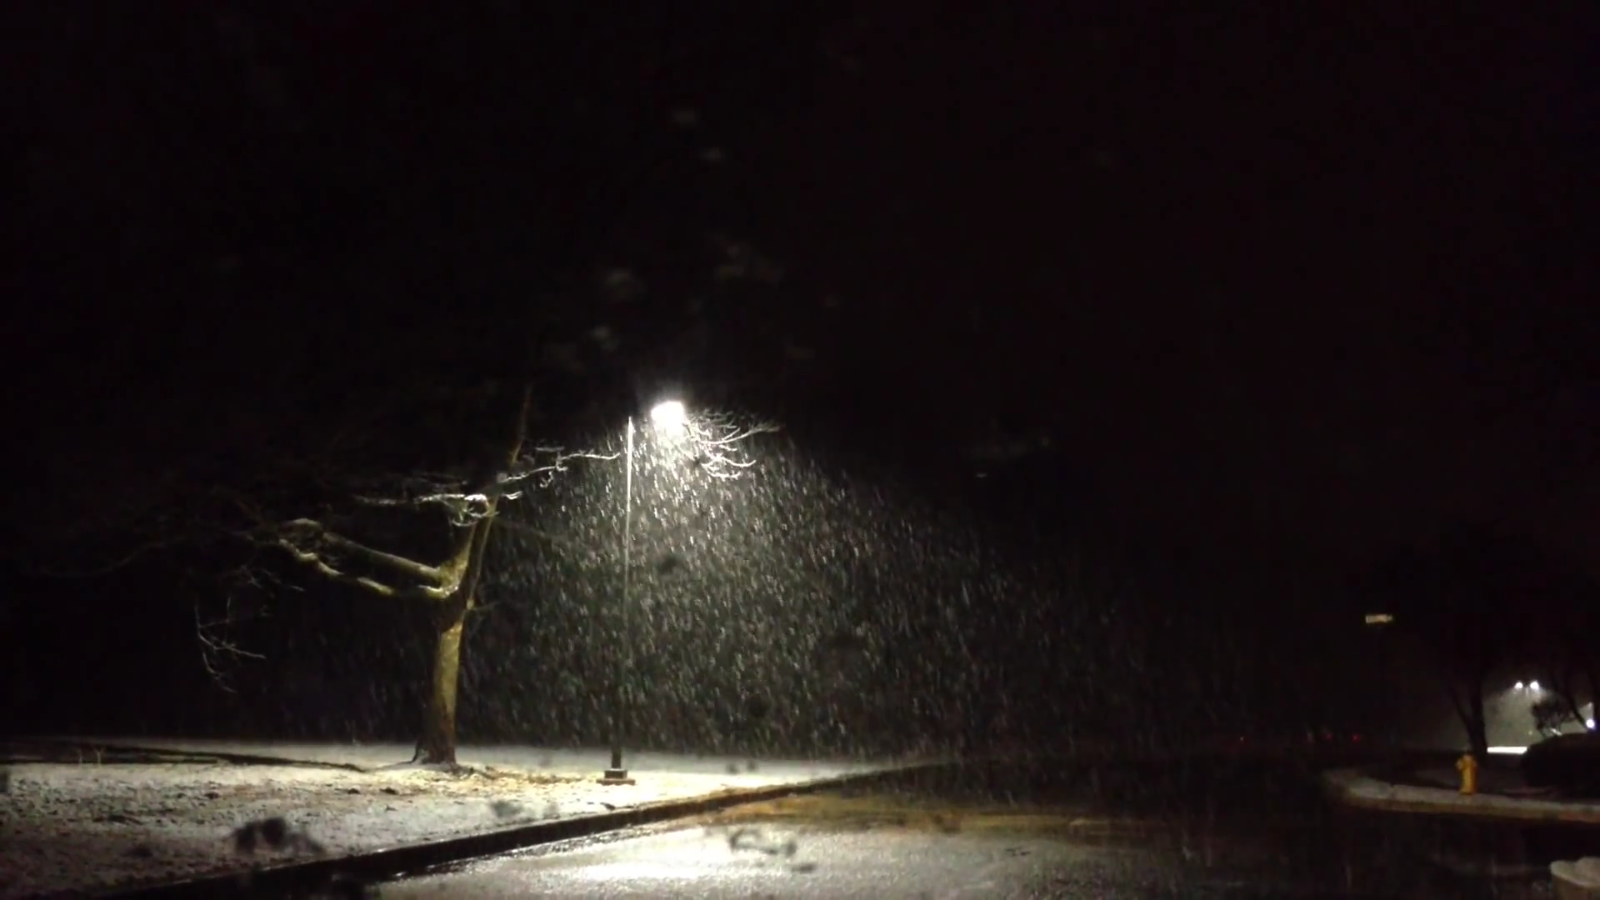
\includegraphics[width=0.9\textwidth]{youtube}
  \caption{\label{fig:youtube} Source: \href{https://www.youtube.com/watch?v=vHZb2xdVTCA}{https://www.youtube.com/watch?v=vHZb2xdVTCA}}
\end{figure}
\noindent
And off we went!



\section{Background}

In Figure~\ref{fig:youtube} and associated video we can identify a couple of elements being present:

\begin{enumerate}
  \item Models for trees and light posts.
  \item Multiple directed light cones.
  \item Snow on the ground.
  \item Snow tumbling through the air.
  \item Shadows cast on the ground.
  \item Snow stuck and falling on the camera lens.
  \item The camera shaking.
\end{enumerate}

All these has some crux, even the most simplest tasks like placing millions of little snow flakes on the screen. Lets look at them in order.


\subsection{Models for trees and light posts}

This first point seems dead simple but can be made quite tedious when one takes into account that models should have textures and preferrably also bump maps baked into them. Seeing as we're not 3D artists by any stretch of the imagination a lot of time can be consumed by such seemingly simple tasks.


\subsection{Multiple directed light cones}

Overlapping of these light cones means either two things:

\begin{itemize}
\item Forward rendering:

  Lighting calculations are made for every object with regards to every light source in the scene. This makes for a complete time complexety of O(nr\_objects * nr\_lights).

\item Deferred rendering:

  Lighting calculations are deferred, as the name implies, until the scene geometry is rendered. This means that depth tests can be used to remove the light calculations of occluded objects.
\end{itemize}

The latter is of course more performant in larger scenes with many light sources. On the other hand its implementation isn't necessarily straight forward.


\subsection{Snow on the ground}

There were some pretty sophisticated models used in the Disney film Frozen \cite{disney-snow}, but we deemed them unfit for real time usage.

The reference video has in itself no moving snow on the ground, but its reasonable to assume that it looks odd if the snow simply falls through the ground.


\subsection{Shadows}

As we can see in Figure~\ref{fig:youtube} the snow casts almost no shadows themselves, this could either be due to the quality of the image or because snow flakes are quite translucent and reemit most of the light touching them. On the other hand the lamp post and the tree creates distinct shadows on the ground.

The most interesting problem here is then to make a distinction between the very smooth shadows that we know, from real life experiences, snow casts on the ground and the very dark shadows of the solid objects. A somewhat ugly solution would be to simply not have the snow flakes cast any shadows.


\subsubsection{Shadow volumes}

One can represent the shadows cast from a solid object when shone upon by a directed light as almost infinitely large geometry in the direction of the light. Wether other solid geometry intersects with these shadow volumes is then used to determine whether or not the objects has a shadow cast on it.

We decided against using shadow volumes as we had absolutely no need for pixel perfect edges for shadows on the ground. On the contrary we want the shadows cast by the snow to be very soft.


\subsubsection{Shadow Maps}

Shadow maps are achieved by rendering a depth map from the viewport of the light source and then using it in the shading of the real render from the camera viewport.


\subsection{Falling snow}

Falling snow is often implemented as some sort of particle system. A particle system of snow is not very hard to implement in the case of calm weather. Particle systems that aim to be very realistic must take into account the fluid dynamics that affect the particles.

\subsubsection{Navier Stokes}

In order to simulate the effect of gusts of wind blowing on the snow Navier-Stokes equations could be used. In \cite{fluid-dynamics} J. Stam describes how the Navier-Stokes equations can be used to implement smokes, clouds and mists in games. Another paper \cite{modeling-falling-accumulating-snow} by Moeslund et. al. also use the Navier-Stokes equations to simulate the wind field that affects the movement of the snow particles.

The movement of a fluid can be described by a velocity field. The Navier-Stokes equations can be applied to calculate the evolution of the velocity field over time. The velocity field can then be used to apply movement to the snow particles. \cite{fluid-dynamics}


\subsection{Sub pixel shadow mapping}
Looks fantastic while being less complex than increasing the resolution of the shadow map equivelently \href{https://www.youtube.com/watch?v=YSQDNy28SDM}{[3]}.



\section{Implementation}

With 3200 fresh lines of code our solution is split up into 10 C files and 10 shader programs. We do geometry instancing for the particle systems, shadow maps for the projection of shadows and proximity based directed lighting.

Our code is organized so that each pair of shaders has a corresponding C-file which deals with all the specifics of that shader, each C-file exposes a single entry point for each shader with the complexities hidden away:

\begin{lstlisting}[label=lst:entry-points,caption= The entry points of each shader pair\, listed in decreasing complexity.]
void drawFull(Model *m, mat4 cameraTransform, mat4 modelTransform,
              mat4 shadowMapTransform, GLuint texture, GLuint shadowMap,
              struct Light* light, vec3 cameraPosition);

void drawModelInstanced(Model *m, mat4 camera, mat4 model,
                        struct Light* light);

void drawSimple(Model *m, mat4 cameraTransform, mat4 modelTransform,
                GLuint texture);

void drawPlain(Model* m, mat4 modelViewProjectionTransform,
               mat4 modelTransform);
\end{lstlisting}

The most simple of our shaders called by \emph{drawPlain} takes only the pointer to a model, a transform from the model coordinate system to that of the camera, and finally a matrix for placing and morphing the model within the world.

If we take a walk into the function in Listing~\ref{lst:drawPlain} it does what you would expect. The code for \emph{drawFull} and all the others are similarily dull.

\begin{lstlisting}[label=lst:drawPlain,caption= The contents of the drawPlain function.]
void drawPlain(Model *m, mat4 cameraTransform, mat4 modelTransform) {
  mat4 modelViewProjectionTransform = Mult(cameraTransform, modelTransform);

  glUseProgram(plainProgram);
  glUniformMatrix4fv(modelViewProjectionLocation, 1, GL_TRUE,
                     modelViewProjectionTransform.m);

  // Vertex positions.
  glBindVertexArray(m->vao);
  glBindBuffer(GL_ARRAY_BUFFER, m->vb);
  glVertexAttribPointer(positionLocation, 3, GL_ GL_FALSE, 0, 0);
  glEnableVertexAttribArray(positionLocation);

  glDrawElements(GL_TRIANGLES, m->numIndices, GL_UNSIGNED_INT, 0L);
  printError("drawPlain()");
}
\end{lstlisting}

What might be of interest is the shader code itself, we will get to that in the following chapters.


\subsection{Lighting and shadow maps}

Something which eased our work was the realization that a camera and a light source have a lot of commonalities:

\begin{lstlisting}[label=lst:lamp-struct,caption=Light source struct]
struct Camera {
  vec3 position;
  vec3 normal;
  vec3 target;
  mat4 projection;
};

struct Light {
  struct Camera camera;
  vec3 intensities;
  float ambientCoefficient;
  float coneAngle;
};
\end{lstlisting}

This made it possible for us to position and rotate the light sources using the normal FPS camera controls we had developed for the camera - merely storing the data kept in a camera and then using it for a light source.

Other than that there is nothing surprising in our implementation of shadow maps. We draw the depth map with the simplest shader possible after which we use the resulting FBO.

Our implementation of shadow maps stems from the course content and an OpenGL article ~\cite{shadow-maps-tutorial} found online.

The vertex shaders does nothing interesting with the geometry, so we will jump straight into the full fragment shader. In Listing~\ref{lst:shader-light-struct} we see the struct passed on to the shader.

\begin{lstlisting}[label=lst:shader-light-struct,caption= The light struct received in the shader.]
uniform struct Light {
  vec3 position;
  vec3 intensities;
  float ambientCoefficient;
  float coneAngle;
  vec3 coneDirection;
} light;
\end{lstlisting}

Using the data passed in as this structure we apply light if the fragment is within the light cone.

\begin{lstlisting}[label=lst:applyLight,caption= Shader function for applying lighting]
vec3 applyLight(Light light, vec3 surfaceColor, vec3 normal,
    vec3 surfacePos, vec3 surfaceToCamera, float shadow) {
  float materialShininess = 1.0;
  vec3 materialSpecularColor = vec3(0.25);

  vec3 surfaceToLight = normalize(light.position - surfacePos);
  float distanceToLight = length(light.position - surfacePos);
  float attenuation = 1.0 / (0.1 + 0.0001 * pow(distanceToLight, 3));

  // Cone restrictions
  float lightToSurfaceAngle = degrees(acos(dot(-surfaceToLight,
    normalize(light.coneDirection))));
  if(lightToSurfaceAngle > light.coneAngle / 2) {
    attenuation = 0.0;
  }

  float diffuseCoefficient = max(0.0, dot(normal, surfaceToLight)
    * 0.5f + 0.5f);
  float specularCoefficient = diffuseCoefficient > 0 ?
    pow(max(0.0, dot(surfaceToCamera, reflect(-surfaceToLight,
      normal))), materialShininess) : 0;

  vec3 ambient = light.ambientCoefficient * surfaceColor.rgb
    * light.intensities;
  vec3 diffuse = diffuseCoefficient * surfaceColor.rgb
    * light.intensities;
  vec3 specular = specularCoefficient * materialSpecularColor
    * light.intensities;

  return ambient + shadow * attenuation * (diffuse + specular);
}
\end{lstlisting}

The last argument passed into the \emph{applyLight} function in Listing~\ref{lst:applyLight} is the output of the \emph{getShadow} function in Listing~\ref{lst:getShadow}.

\begin{lstlisting}[label=lst:getShadow,caption= The shader function figuring out whether the fragment is in the shade.]
float getShadow(int index) {
  // Perform perspective division to get the actual texture position
  vec4 shadowCoordinateWdivide = lightSourceCoord[index] / lightSourceCoord[index].w;

  /* Used to lower moire' pattern and self-shadowing
   * The optimal value here will vary with different GPU's
   * depending on their Z buffer resolution.
   */
  shadowCoordinateWdivide.x -= 0.00001;
  shadowCoordinateWdivide.y -= 0.00001;
  shadowCoordinateWdivide.z -= 0.00005;

  float shadow = 1.0; // 1.0 = no shadow
  for (int i = 0; i < 4; i++) {
    int randomIndex = int(4.0 * random(gl_FragCoord.xyy, i)) \% 4;
    float distanceFromLight = texture(shadowMap[index], shadowCoordinateWdivide.st
                              + poissonDisk[randomIndex] / 1000.0).x;
    distanceFromLight = (distanceFromLight-0.5) * 2.0;

    if (lightSourceCoord[index].w > 0.0)
      if (distanceFromLight < shadowCoordinateWdivide.z)
        shadow -= 0.001 / (shadowCoordinateWdivide.z - distanceFromLight);
  }
  shadow = clamp(shadow, 0.2, 1.0);
  return shadow;
}
\end{lstlisting}

As is visible in Listing~\ref{lst:getShadow} we make four pseudo-randomly scattered samples for each fragment. This results in the dithering which can be seen in Figure~\ref{fig:dithering}. It doesn't look very pretty close up, but at a distance it smooths out an otherwise straight edge.

\begin{figure}[ht]
  \centering
  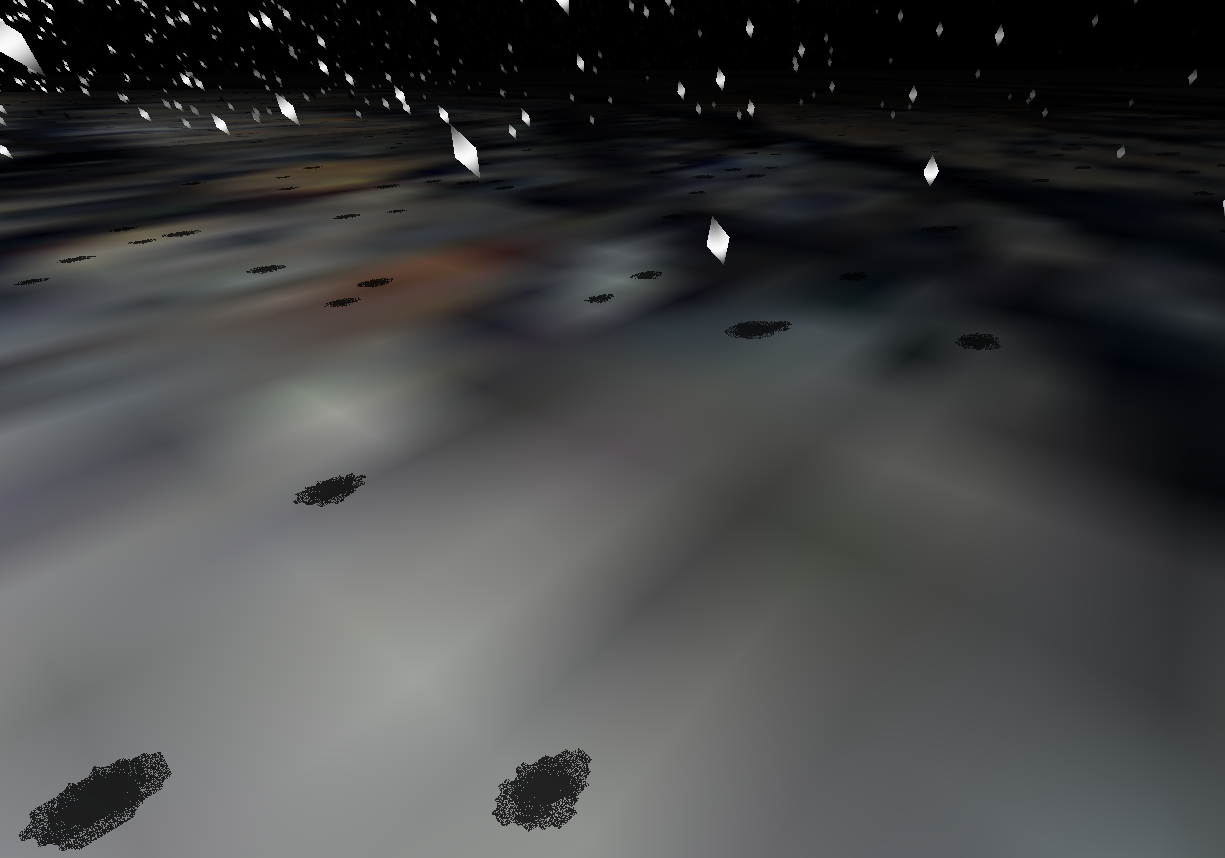
\includegraphics[width=0.9\textwidth]{dithering}
  \caption{\label{fig:dithering} The effect of the pseudo random shadow map samples.}
\end{figure}

\subsection{FBO debugging}

We implemented the display of FBO's so that we could see what was drawn into them. As we can see in Listing~\ref{lst:fbo-code} we are able to reuse our normal drawing code for the debugging.

\begin{lstlisting}[label=lst:fbo-code,caption= Switching between the FBO's]
int displayFBOKeyIsDown = keyIsDown('f');
if(displayFBOKeyWasDown && !displayFBOKeyIsDown)
  displayFBO = (displayFBO + 1) % (NR_STREET_LIGHTS + 1);
displayFBOKeyWasDown = displayFBOKeyIsDown;
if(displayFBO)
  drawSimple(modelPlane, Mult(S(.04, .04, .04), Rx(45)), IdentityMatrix(),
    fbos[displayFBO - 1]->depth);
\end{lstlisting}

This places a square in front of the camera displaying the depth buffer we want to inspect:

\begin{figure}[ht]
  \centering
  
\includegraphics[width=0.9\textwidth]{fbo}
  \caption{\label{fig:fbo-image} The depth buffer from a street light.}
\end{figure}

Everything not completely white in Figure~\ref{fig:fbo-image} will be considered shadowed.

\subsection{Snowfall}
Even though the geometry shader is preferable for particle systems, we chose to implement the vertex generation and movement on the CPU because of simplicity. If we instead had utilized the geometry shader we could have increased the number of snow particles without a major performance hit.

The vertex shader for the snowfall contains nothing of interest. The fragment shader is very similar to the full shader (which is used to render the street lamp), the most visually apparent difference is that the snow particles are rendered without shadows.

The model for the snow particles is a double cone as shown in Figure~\ref{fig:dcone-image}. The idea of using a double cone comes from a paper by N. Wang et. al. \cite{snow-rain}. The model is rendered with a texture which makes the top and bottom edges transparent. N. Wang et. al. applies motion blur to elongate the particles, which we believe would improve our result further. We did not have the time to implement that however.
\begin{figure}[H]
  \centering
  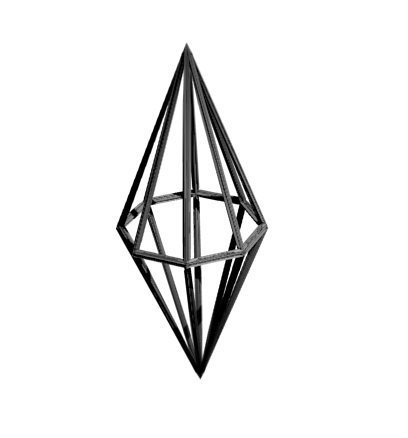
\includegraphics[width=0.3\textwidth]{dcone}
  \caption{\label{fig:dcone-image} The depth buffer from a street light.}
\end{figure}



\section{Issues}

Not only did we have issues on our own, the project had a lot of issues too.

\subsection{Detangling global state}

We have probably refactored the codebase completely somewhere around three times, trying to untangle it from iself. The code we started out with, mostly based on old lab, had a lot of global state on the heap which was modified in a lot of different places. In a lot of cases we could justify keeping for example vectors or 4 by 4 matrixes on the stack, the functional purity was more important than the minute performance gains.

\subsection{Shadow buffer bugs}

We ended up wasting about a week doing nothing but trying to debug a fully working implementation of shadow maps, only that it did not render correctly on the specific hardware we were developing it on. The bug resulted in flimmering shadows.

We failed to track down what actually caused the bug, although we know the fault happend when rendering the shadow map to the FBO. It would have been nice if we could find the cause, so that we could fully understand the underlying problem. We did learn a lot while trying to figure this one out, but in the end the most important lesson was to try on different hardware.

TODO: Add screenshot of the bug. (worked on NVIDIA NVS 4200M which is similar to a GT520M)

The lesson learnt is to try the code on more than one machine.



\section{Conclusions}

``The wrong man in the right place, can make all the difference in the world'' as we know from the writings of our Lord and Saviour Gabe Newell in the annals of Half Life 2. In our project we absolutely encountered a lot of very basic issues such as placing items in the world, simply because we had to write that logic from scratch. More than anything else we have realised the wisdom in the quote ``Write a game, not a game engine''. If we were to actually make a computer game at any point in our lives we will, with the experience of this course in our backpack, seriously consider utilizing existing libraries or existing game engines. Because if you do not you end up, like us, never getting to work on the stuff you are actually interesting in; only working on the tedious neccecities which facilitate what you want to do.

In the end we didn't have enough time to implement Navier Stokes equations or anything more fancy than pseudo random rotations applied to our snow flakes which is somewhat disappointing. We ended up spending a lot of time working on light and shadows when it was the snow dynamics we really wanted to work on.

In Figure~\ref{fig:result} we can see a screen capture of the resulting scene. Things of note are the thousands of tiny snow flakes casting shadows on the ground. The light cones of the street lights do intersect and add up to each other on the same ground object.

\begin{figure}[ht]
  \centering
  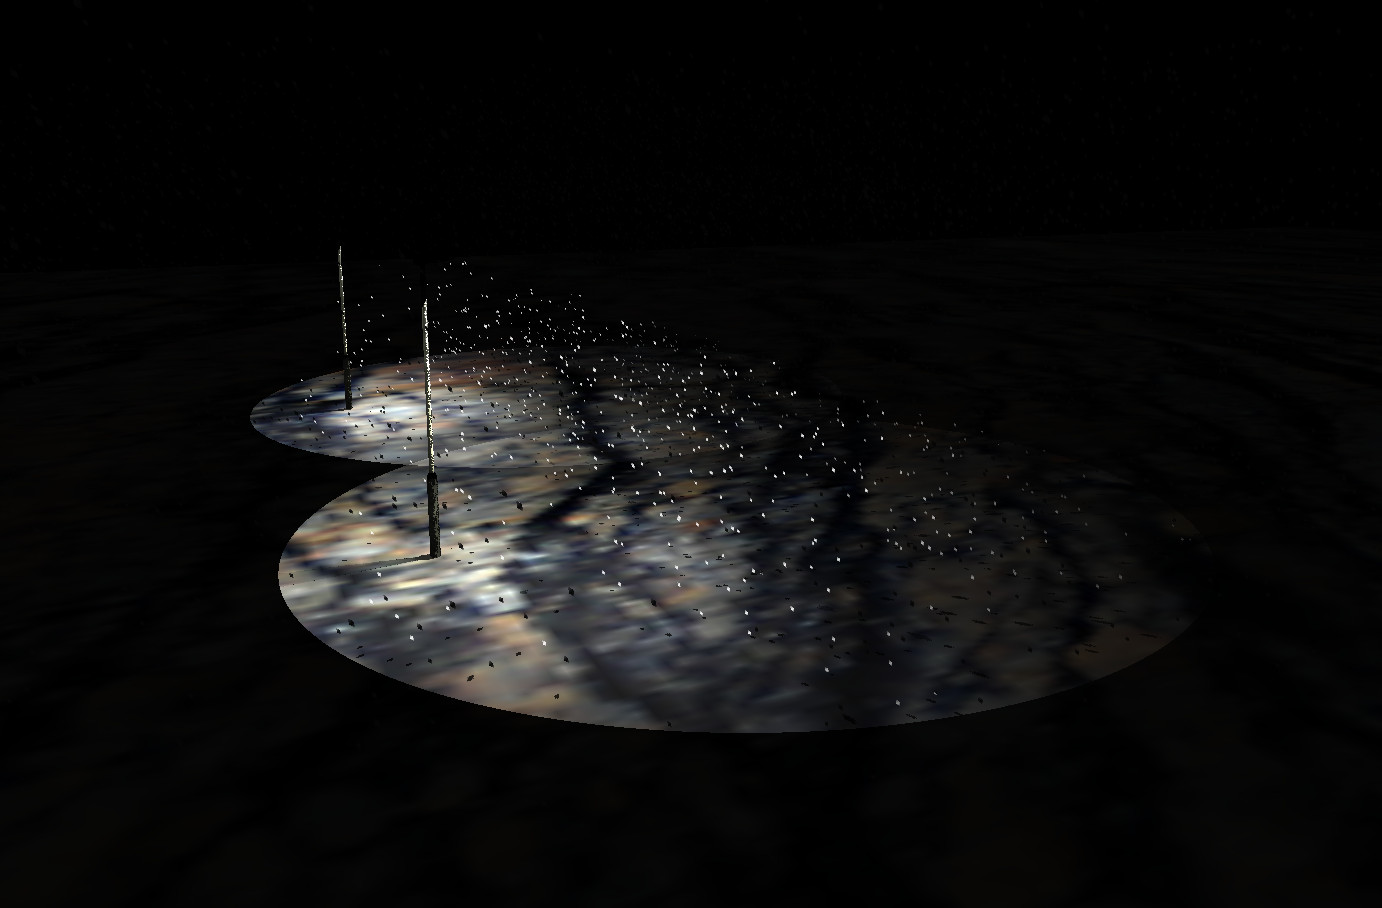
\includegraphics[width=0.9\textwidth]{result}
  \caption{\label{fig:result} Our OpenGL snow scene.}
\end{figure}

You can also see a short video on \href{YouTube}{TODO!}

\newpage

\begin{thebibliography}{9}
  \bibitem{shadow-maps-tutorial}
    Opengl-tutorial.org.
    \emph{Tutorial 16 : Shadow mapping}.
    2016.
    Available: \url{http://www.opengl-tutorial.org/intermediate-tutorials/tutorial-16-shadow-mapping/.}
    Accessed: 2016-01-20

  \bibitem{disney-snow}
    Stomakhin, Alexey, Craig Schroeder, Lawrence Chai, Joseph Teran, and Andrew Selle.
    \emph{A Material Point Method for Snow Simulation.}
    TOG 32.4 (2013): 1

  \bibitem{fluid-dynamics}
    Stam, J. (2003).
    \emph{Real-Time Fluid Dynamics for Games.}
    Proceedings of the Game Developer Conference, 18(11), 17. doi:10.1.1.12.6736

  \bibitem{snow-rain}
    Wang, N., \& Wade, B. (2004).
    \emph{Rendering Falling Rain and Snow.}
    ACM SIGGRAPH 2004 Sketches, (sketches 0186), 14. doi:10.1145/1186223.1186241

  \bibitem{modeling-falling-accumulating-snow}
    T.B. Moeslund, C.B. Madsen, M. Aagaard, and D. Lerche
    \emph{Modeling Falling and Accumulating Snow}
    Vision, Video and Graphics (2005)

\end{thebibliography}


\end{document}
